\textbf{Consider again the approximation of $f(x)=3/(5−4cos(x))$, $x\in[-\pi,\pi]$. Let $N$ be the number of nodes in Fourier and polynomial interpolation of this function.
\begin{enumerate}[label=\alph*)]
\item Plot the error as a function of $N$ (on the same figure) for both Chebyshev and Fourier. Notice
that Fourier converges at a faster rate in this case.
\item Now consider that maximum spacing between nodes: $h=max|x_{i+1}-x_i|$. Plot the error for
polynomial and Fourier approximations as a function of $h$ and notice that the rates of convergence
are now nearly the same.
\item Show that the ratio $h_{cheb}/h_{Fourier}$ is about $\pi/2$.
\end{enumerate}
$~$}
\newline

For the first part we look at the next figure. We can see that, in fact, Fourier converges at a faster rate in this function.

\begin{figure}[H]
\centering
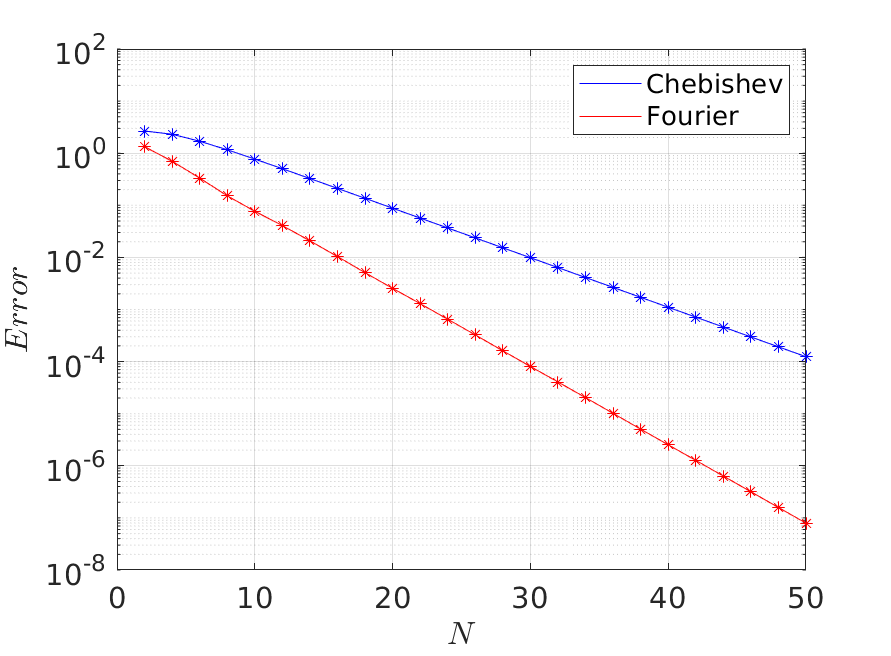
\includegraphics[scale=0.75]{P7_a.png}\caption{Convergence of the Chebyshev and Fourier interpolants to $f(x)= \frac{3}{54\cos{x}}$.}
\end{figure}

We continue by scaling the Chebyshev points to be withing $[-\pi,\pi]$ and calculate $h$ for both Chebishev and Fourier, for each $N$. We obtain the following figure, which shows that the rates of convergence are nearly the same.
\begin{figure}[H]
\centering
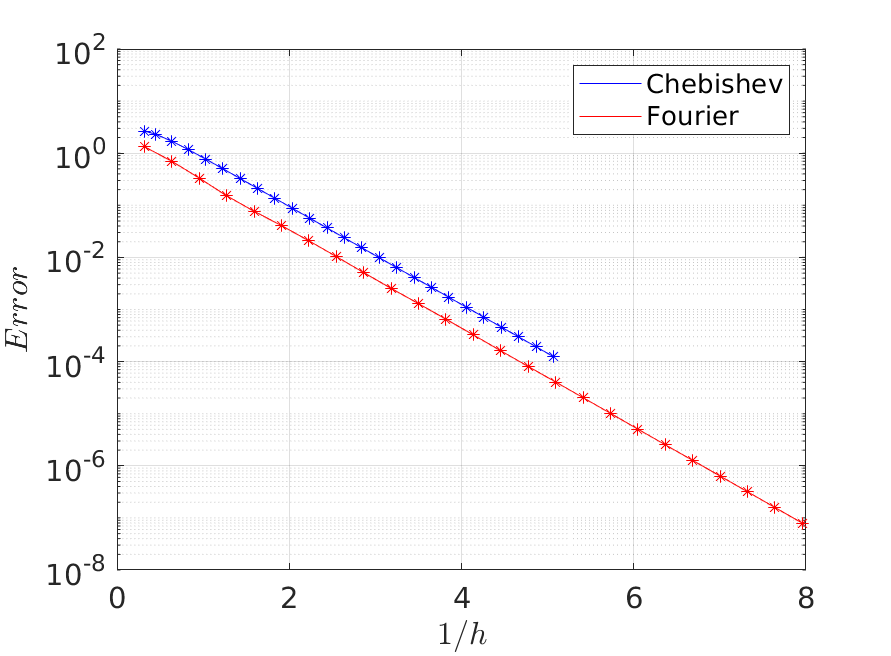
\includegraphics[scale=0.75]{P7_b.png}\caption{Convergence of the Chebyshev and Fourier interpolants to $f(x)= \frac{3}{54\cos{x}}$.}
\end{figure}

Lastly, in the following figure we see that, once is large enough, $h_{Cheb}/h_{Fourier}\approx \pi/2$.

\begin{figure}[H]
\centering
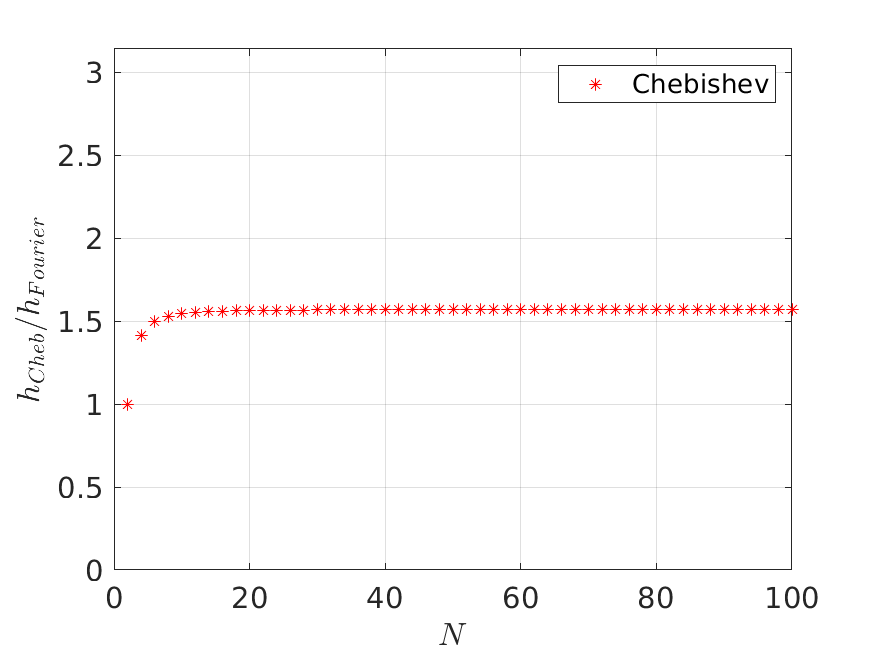
\includegraphics[scale=0.75]{P7_c.png}\caption{$h_{Cheb}/h_{Fourier}$ for $f(x)= \frac{3}{54\cos{x}}$.}
\end{figure}

\subsection*{Matlab code for this problem}
\begin{verbatim}
%% Problem 7
close all
f = chebfun('3/(5-4*cos(x))',[-pi,pi]);
plot(f)
grid on
N = 2:2:50;
for k = 1:length(N)
    fcheb = chebfun('3/(5-4*cos(x))',[-pi,pi],N(k));
    ffour = chebfun('3/(5-4*cos(x))',[-pi,pi],N(k),"trig");
    errcheb(k) = norm(f-fcheb,inf);
    errfour(k) = norm(f-ffour,inf);
    % b
    [~,x] = cheb(N(k)); x = pi*x;
    hcheb(k) = max(abs(x(2:end)-x(1:end-1)));
    hfour(k) = 2*pi/(N(k));
end
% a
figure
semilogy(N,errcheb,'b',N,errfour,'r')
hold on
semilogy(N,errcheb,'b*',N,errfour,'r*')
grid on
xlabel('$N$','interpreter','latex')
ylabel('$Error$','interpreter','latex')
set(gca,'fontsize',labelfontsize)
legend('Chebishev', 'Fourier')
txt='Latex/FIGURES/P7_a';
saveas(gcf,txt,figformat)
% b
figure
semilogy(hcheb.^(-1),errcheb,'b',hfour.^(-1),errfour,'r')
hold on
semilogy(hcheb.^(-1),errcheb,'b*',hfour.^(-1),errfour,'r*')
grid on
xlabel('$1/h$','interpreter','latex')
ylabel('$Error$','interpreter','latex')
set(gca,'fontsize',labelfontsize)
legend('Chebishev', 'Fourier')
txt='Latex/FIGURES/P7_b';
saveas(gcf,txt,figformat)
% c
figure
plot(N,hcheb./hfour,'r*')
grid on
axis([0 50 0 pi])
xlabel('$N$','interpreter','latex')
ylabel('$h_{Cheb}/h_{Fourier}$','interpreter','latex')
set(gca,'fontsize',labelfontsize)
legend('Chebishev', 'Fourier')
txt='Latex/FIGURES/P7_c';
saveas(gcf,txt,figformat)
\end{verbatim}